\section{Evaluation}
\label{sect:apner_results}
We first report on a study in which we evaluate the generation of candidate entities using vector distances from representative (frequently used) entities. 
%\logan{Would using "candidate entities" rather than "distance candidates" make more sense?}
%\logan{If F\ref{fig:current} describes your setup. Why not reference it here?}\roselyne{That is the set up for the active learning but I also evaluate the candidate generation, so I think for now, I'll leave it out but see if I refer to it in the sections below.}
We then discuss the results of initial classification and subsequent four rounds of active learning using multiple word vector classifiers and our three sampling strategies: random, UBS, and Distance UBS.
Finally, we experiment with word representations enhanced with character-level information using FastText~\cite{bojanowski2016enriching,joulin2016bag}.

In this work, we evaluate extraction accuracy in terms of precision and recall.
\emph{Precision} refers to the fraction of predicted
positives that are labeled correctly and
\emph{recall} to the fraction of actual positives that
are labeled correctly.

\subsection{Dataset}\label{sec:dataset}

We work with a corpus of \num{1690} full-text publications in HTML format from \textit{Macromolecules}, 
a relevant journal in polymer science.
These documents comprise \num{381947} sentences and \num{9229417} (\num{253195} unique) words or ``tokens,''
of which \num{23205} pass the NLP filter of Section~\ref{sec:filter}.

From this corpus, 
we set aside a test set of 100 documents with  \num{22664} sentences and \num{508391} (\num{36293} unique) tokens,
of which \num{9656} pass the NLP filter.
We engaged six experts to identify all one-word polymer names in this test set,
a process that produced 467 unique one-word polymer names.
We use these 467 names as a gold standard in subsequent subsections; we automatically label all NLP-filtered strings from the 100-document test set using these manually extracted names.


%\logan{What part of this data can we release, if any?}\roselyne{Hong and I are working on a dataset following a schema we discussed for release, I think we talked about it but didn't update you guys back. However it's more like NLP datasets, where we are releasing sentences with entities and not this exact dataset}

\subsection{Seed Entities}\label{sec:wes}
Recall from Section~\ref{sec:wordembeddings} that polyNER uses the
Word2Vec word embedding tool to compute a word vector for each word.
In order to maximize the number of actual entities in the dataset\textemdash and the ratio of target to non-target entities\textemdash in the initial set of labels,
we explore how the choice of seed entities
impact the number of target entities retrieved.
%XXX_IAN don't understand next sentence
While we cannot expect meaningful classification using only positive examples, 
given the imbalance in the whole dataset, we aim to select the Word2Vec parameters that yield the highest ratio of polymers in this initial batch of candidates.

%\ian{Maybe the following would be simpler if written as follows. This seems to say what you are trying to say?: 
%``We use the 467 gold standard polymer names identified by experts in our 100-document test set to
%evaluate the performance of different word embedding settings.
%Specifically, for each choice of settings that we want to evaluate,
%we determine the \num{10000} distance candidate vectors that are most similar to the representative entity vectors 
%and report what fraction of the 467 gold standard names are included in that \num{10000}.
%We use lower-case exact string matching between the gold standard polymer names and the proposed distance candidate strings to determine if a candidate is a polymer.}
%\roselyne{Thank you. I want to justify the number 10000, will rephrase because your text is better but it doesn't answer the question why 10000 necessarily}
%\ian{This section is just about seed entities, which only applied to Distance UBS. So it should renamed, I think?}

In the experiments that follow,
we use the 467 gold standard polymer names identified by experts in our 100-document test set to
evaluate performance with different seed entities.
Specifically, for each choice of seed entities that we want to evaluate,
we determine the \num{10000} NLP-filtered words with vectors closest to the seed entity vectors, 
and report what fraction of the 467 gold standard names are included in that \num{10000}.
We use lower-case exact string matching between the gold standard polymer names and the proposed distance candidate strings to determine if a candidate is a polymer.
%To estimate the entity-richness of our large pool of distance candidates and since we do not have manually extracted data for the entire corpus, we create a list of \num{10000} distance candidate vectors most similar to our representative entity vectors and report the fraction of gold standard polymers extracted. 
%In our gold-standard of publications, there are $\sim$5 polymers per document (\num{8450} polymers for \num{1690} documents). Thus, we expect a fraction of the polymers found in the 100 gold standard documents to be extracted in the \num{10000} candidates most similar to our seed entities.
%\ian{I have no idea what you are trying to say here $\ddot\smile$. You say ... ``our gold-standard of publications ... 1690 documents'', but previously you define the gold standard as being 100 documents.}
%\logan{This is confusing. Why are we using a model to estimate the total population of the polymers and not just assuming the gold-standard is a representative sample?}\roselyne{ok, 467/100)}
%We evaluate the entity-richness of polymers in this pool of candidates by measuring the percentage of the 467 manually extracted polymer names that it yields;
%we use lower-case exact string matching between the gold standard polymer names and the proposed distance candidate strings to determine if a candidate is a polymer.

%\subsubsection{Seed entities}
%We investigate how the choice of seed entities affects performance.
In previous work using the same corpus~\cite{tchoua2016hybrid,tchoua2016hybridi}, 
we built a dictionary of polymer names by using a rule-based approach and aggregating synonyms across ChemDataExtractor records. (A record consists of all information found about a chemical entity in a document.)  
Here we use this dictionary to identify the 10 most frequently occurring polymers in our corpus and their acronyms.
%\ian{Table says ``most frequent,'' text says ``most common.'' Be consistent.}\roselyne{check everywhere.}
%Experts can also suggest these entities based on prior knowledge.
We assume that frequent polymers provide a large number of sentences that illustrate context in which polymers are commonly used.
%\logan{Do you think it would be better to use the gold standard, where we have certainty of the labels, to estimate the most-frequent polymers?}\roselyne{we used the entire corpus, we know the most frequent polymers}
Hence, we first test the most frequent, the three most frequent, and the ten most frequent polymers as seed entities.
%\logan{The circularness of this strategy makes me uncomfortable. We use an NER model to determine the initial training set for the NER model? How would you address this criticism?}\roselyne{not sure I understand how I am using an NER model to determine the NER model, I'm just testing with various seed entities. As you suggested before, experts can give this info, or we can just measure the frequency of a few known entities. Added a line about this so that no prior work is needed.}
We also experiment with including and excluding their acronyms as additional seed entities.
(Note that this modest set of 1, 3 and 10 seed entities could also be suggested by an expert.)

Rows 1--6 of Table~\ref{tab:candidate_generation} shows the results for these experiments.
When using \textit{polystyrene} (the most frequently used name) as a seed entity, 
the candidates contained 33.6\% of the 467 gold standard polymers.
%\logan{Another potential criticism: Would I need a gold standard to build the NER method? I thought your method is supposed to help me avoid having to do the work for generating a gold standard?}\roselyne{There is no way to evaluate if you don't have a gold standard is there?}
We note a 2\% increase in the fraction of polymers retrieved when using both \textit{polystyrene} and \textit{PS}, 
when compared to using \textit{polystyrene} alone. % (37.69\%).
%\logan{Is this an important detail? Why does it need to stay [I think this section is a little dense]}\roselyne{well, before Kyle thought this was a bit vague, so I added lots of numbers, I may come back and remove this}\roselyne{Removing details from here}
The fraction of polymers increases by 10\% when we use three representative entities 
%(from 33.55\% to 46.9\% and 47.97\% with acronyms); 
(the three most frequent polymers in our datasets are \textit{polystyrene}, \textit{poly(methyl methacrylate)}, and \textit{polyethylene}), % and their acronyms (\textit{PS}, \textit{PMMA} and \textit{PE})
but by less than 1\% when using 10 instead of three entities. %, from 47.97\% for three frequent polymers with acronyms to 48.39\% for ten frequent polymers with acronyms.
These results suggest that there is little value to using more than a few seed entities.

\begin{table}[ht!]
\centering
\caption{Fraction of gold standard polymer names in the \num{10000} entities that are closest,
by word vector distance, to various sets of seed entities.\label{tab:candidate_generation}}
\vspace{2ex}
%[35.55, 37.69, 46.9, 47.97, 46.47, 48.39, 46.68, 36.4]
\setlength\tabcolsep{3pt}
\begin{tabular}{|C{0.1in}|C{2.4in}|C{0.6in}|}
 \hline
\textbf{\#} & \textbf{Seed entities} & \textbf{Fraction of polymers extracted}  \\
\end{tabular}
\begin{tabular}{|C{0.1in}|R{2.4in}|L{0.6in}|}
\hline\hline
 1 &    Polystyrene & 35.6\% \ \ \ \  \\
\hline
 2 &    Polystyrene, with acronym PS & 37.7\% \ \ \ \ \\
\hline
 3 &    Three most frequent polymer names & 46.9\% \ \ \ \ \\
\hline
 4 &    Three most frequent polymer names, with acronyms &  48.0\% \ \ \ \ \\
\hline
 5 &    10 most frequent polymer names & 46.5\% \ \ \ \ \\
\hline
 6 &    10 most frequent polymer names, with acronyms & 48.4\% \ \ \ \ \\\hline
\hline
 7 &    $\chi$DB polymer names & 46.7\% \ \ \ \ \\
\hline
  8 &  crowDB polymer names    & 36.4\% \ \ \ \ \\
\hline
\end{tabular}
\end{table}

To further explore whether using larger numbers of seed entities may increase the fraction of polymers retrieved,
we conducted a second set of experiments.
We have built a small database of polymer properties ($\chi$DB) in previous work~\cite{tchoua2016hybrid,tchoua2016hybridi}. 
Our corpus of \num{1690} publications included 111 out of 175 $\chi$DB polymers.  
We also scraped CrowDB, which lists some polymers and their properties at \url{http://polymerdatabase.com/} for polymer names; 32 out of 295 scraped polymer names were found in our corpus.
We measure how many of our gold standard polymers are identified when
these 111 and 32 polymer names are used as seed entities, 
with results shown in rows seven and eight of Table~\ref{tab:candidate_generation}.
These results confirm that using more entities does not increase the yield of polymers.
%as some polymers have low frequency in the corpus, words that are most similar are less likely to be targets.
Thus, in all subsequent experiments, we use the three most frequent polymers and their acronyms as seeds. 
%\logan{I think the metric we use for choosing an algorithm here (fraction of entries in the training set) is too indirect. Why not use the performance of the initial ML model to rate how good the training set is? A hypothetical concern with the metric as well: Does your current metric mean a pool with 100\% polymers would be the best? Wouldn't that lead to the same problem of imbalance as having no polymers?}
%\roselyne{how about just 50-50\% what would be wrong with training on such a dataset, why should we reach 100\%, maybe I should add somewhere that this is a good ration, or anywhere higher than 10\%. I will consider that next time, but I think this made sense to me, increase from 5\% to reduce imbalance. I mentioned in the discussion that we evaluated based on entity richness but could evaluate in terms of discrimination, it's a lesson learned.}


%\kyle{perhaps better as a table. The long labels are hard to read}\roselyne{ok}
%\begin{figure*}
%\centering
%\begin{minipage}[b]{.4\textwidth}
%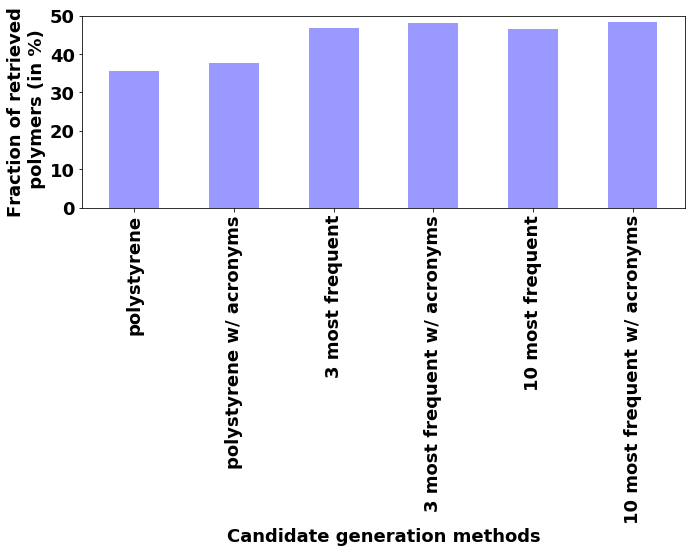
\includegraphics[trim=0in 0.1in 0.1in 0.in,clip,width=1.0\textwidth]{figures/candidate_generation_method1.png}
%\caption{\label{fig:cand_generation1} Fraction of polymer retrieved for various candidate generation methods using most common, three most common and ten most common polymer names as seed entities.
%}
%\end{minipage}\qquad
%\begin{minipage}[b]{.4\textwidth}
%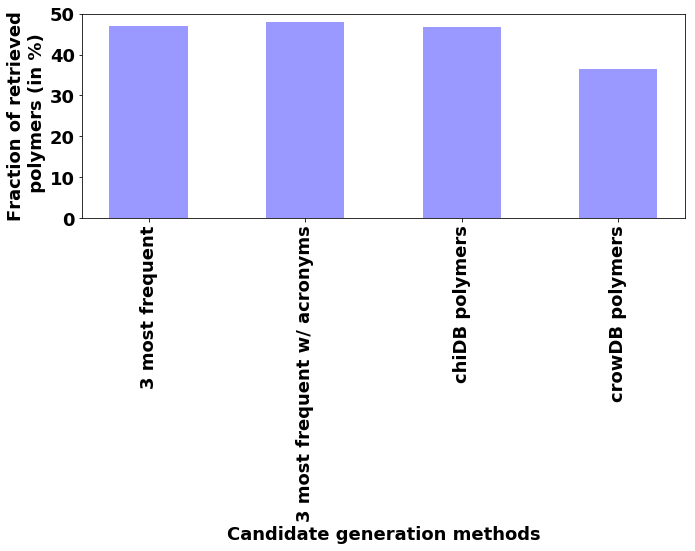
\includegraphics[trim=0in 0.1in 0.1in 0.in,clip,width=1.0\textwidth]{figures/candidate_generation_method2.png}
%\caption{\label{fig:cand_generation2} Fraction of polymer retrieved for various candidate generation methods using three most common (with and without acronymss), $\chi$DB and CrowDB polymer names as seed entities.  
%%\kyle{Not sure this needs to be a separate graph?}
%}
%\end{minipage}
%\end{figure*}
%Together
%[35.55, 37.69, 46.9, 47.97, 46.47, 48.39, 46.68, 36.4]
%[35.55, 37.69, 46.9, 47.97, 46.47, 48.39]
%\begin{figure}[!t]
%\centering
%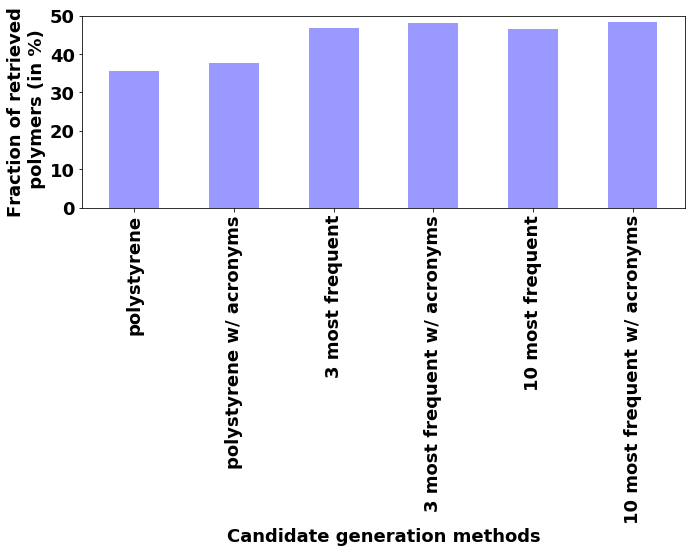
\includegraphics[trim=0in 0.1in 0.1in 0.in,clip,width=3.5in]{figures/candidate_generation_method1.png}
%\caption{\label{fig:cand_generation1} First set of experiments with seed entities showing noticeable improvement from 1 to 3 and less improvement from 3 to 10 seed entities.
%}
%\end{figure}
%[46.9, 47.97, 46.68, 36.4]
%\begin{figure}
%\centering
%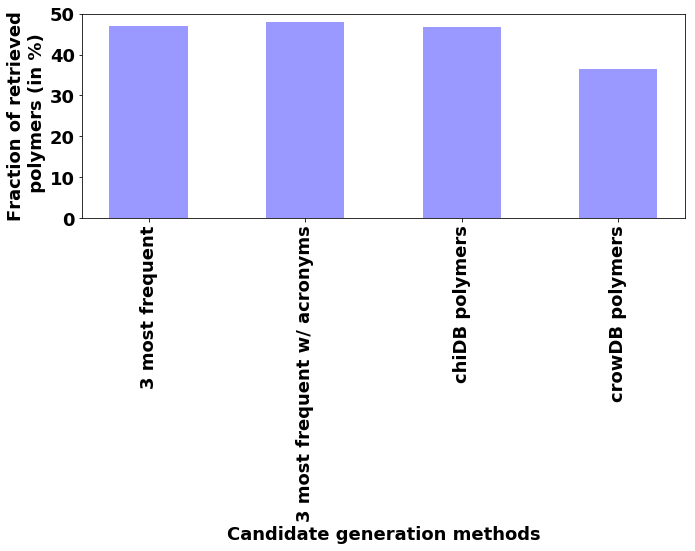
\includegraphics[trim=0in 0.1in 0.1in 0.in,clip,width=3.5in]{figures/candidate_generation_method2.png}
%\caption{\label{fig:cand_generation2} First set of experiments with seed entities showing that using more polymers as seed entities does not necessarily enrich the pool of distance candidates.
%}
%\end{figure}

%\subsubsection{Word Embedding Window and Size Parameters}
%We generate a pool of \num{10000} candidates most similar to the three most frequent polymers and their acronyms from a test corpus of \num{1690}, excluding any token found in our test documents. 
%As previously mentioned, to measure the entity-richness of our dataset, we compute the fraction of polymers retrieved using the distance measure to our representative entities in the  \num{10000} candidates.
%%We measure the impact of the \textit{window} and \textit{size} on the fraction of polymers extracted from the gold standard in the list of \num{10000} candidates most similar to our representative entities. 
%%\logan{Where are the 10k candidates from again? Could we reference this set by its purpose rather than its size?}\roselyne{Done I think.}
%%\logan{Need a reason why this is important? Also, this statement again raises my concern about using "fraction extracted from gold standard" as a metric for quality of the initial training set?}\roselyne{same answer as above, trying to increase balance in dataset.}
%The \textit{window} represents the maximum distance between the current and predicted word within a sentence. In other words, it represents the number of words before and after each word considered by the neural network to generate a vector representation for that word. 
%For each parameter setting, we measure the yield of polymers ten times for each window and vector size setting.
%We observe slightly higher fraction of polymers retrieved for window sizes of 1 and 2. The yield subsequently decreases and more noticeably with window size larger than 5 (see Figure~\ref{fig:window_size}).
%The \textit{size} determines the size of the word vector (features for our classifier).
%We varied this parameter between 100 and 500.
%The average yield of polymer names was measured at 49.3 with a standard deviation of less than 1\% (see Figure~\ref{fig:vector_size}).
%We conclude that the vector size does not impact the fraction of polymers retrieved during the distance candidate generation.
%[49.67880085653105, 49.25053533190578, 49.46466809421842, 49.46466809421842, 48.82226980728051]
%\logan{Need a concluding sentence?}

%\begin{figure}
%\centering
%%\begin{minipage}[b]{.4\textwidth}
%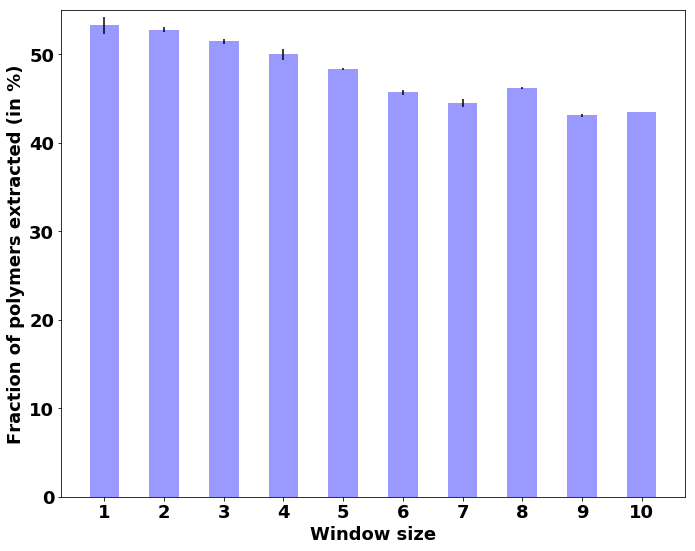
\includegraphics[trim=0in 0.1in 0.1in 0.in,clip,width=3.5in,height=2.5in]{figures/window_size.png}
%\caption{Impact of varying window size on fraction of polymers retrieved.}\label{fig:window_size}
%%\end{minipage}\qquad
%%\begin{minipage}[b]{.4\textwidth}
%%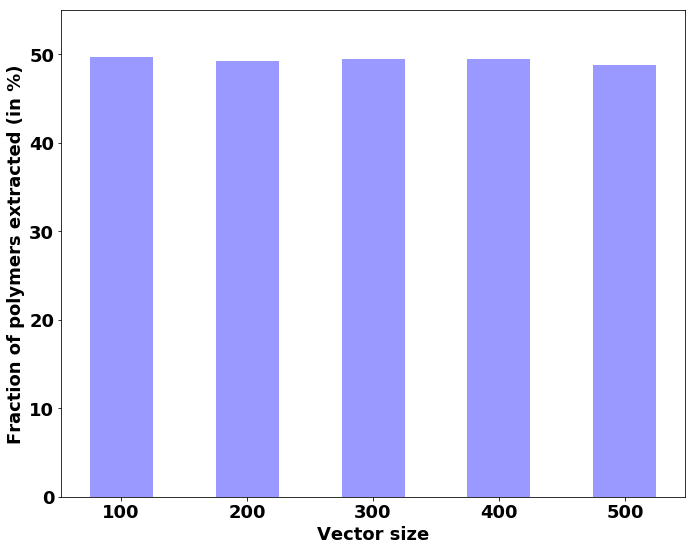
\includegraphics[trim=0in 0.1in 0.1in 0.in,clip,width=1.0\textwidth]{figures/vector_size.png}
%%\caption{Impact of varying vector size on fraction of polymers retrieved. \logan{Can we combine this with F\ref{fig:window_size}? (If we keep it) }}\label{fig:vector_size}
%%\end{minipage}
%\end{figure}
 %\kyle{Not sure this fig is worth including}\roselyne{Agreed that it's not so interesting but i think it goes with the windows one and i will combine the two figures you think should be together.}\roselyne{May remove as paper gets longer}

%\roselyne{We can put labeling here, or maybe before last results, but I think it should be before the discussion and the final main result}
\subsection{Labeling}\label{sec:labeling}
We conduct some experiments to estimate labeling time. 
We ask two polymer scientists to label 200 candidates from a subset of our corpus.
One expert reports 30 minutes, the other 45 minutes. We overestimate the time to label 200 candidates at one hour of expert time.
Based on user feedback, we also improve the labeling Web interface after the above mentioned test rounds to further facilitate and speed up labeling.
For example, we increase the number of example sentences available to provide context, to decrease the number of occurences in which experts have to look up original publications for candidates.
We also increase the size of checkmarks to make it easier to reject erroneous candidates.
%Having performed these initial tests, and considering that expert time is expensive, we allow annotators to save their progress and come back to labeling anytime within a week's time. \roselyne{Is this only going to add confusion?}
In the initial labeling round, 
we perform crosschecking for 10\% of the batch of labels. 
We confirm agreement between labels for all but one of 20: an agreement rate of 95\%.

\subsection{The Initial Classifier}
Recall from Section~\ref{sec:bootstrap} that we use an initial set of 200 NLP-filtered entities that are close
to seed entities to bootstrap our labeling process.
Once those data are labeled by our experts, 
we use 80\% to train a KNN classifier, validating on the remaining 20\%. 
We then test this \textit{initial classifier} against all \num{9656} NLP-filtered candidates in the 100-document test set,
which as noted in Section~\ref{sec:dataset} contain \num{467} polymers.
Results are shown in Figure~\ref{fig:knn_init}.
Its Receiver Operating Characteristic (ROC) curve
shows better-than-random behavior, with an area under curve (AUC) of 0.62. 
 %shows the Receiver Operating Characteristic (ROC) curve for the initial classifier with highest recall when evaluating on the test corpus.
%\logan{I do not like this as a topic sentence because it doesn't offer any indication of what to draw from the figure. I prefer ones that are "We found that X, as shown in Figure Y." Topic sentences with some editorial comments worked in help keep the narrative of the purpose of your study alive.}
%The ROC plot is an evaluation measure that is based on two basic evaluation measures: specificity (true positive rate) and sensitivity (true negative rate).
%Sensitivity is the same as recall. Specificity is a measure of the true negative rate (the proportion of actual negatives that are correctly identified as such).
%A classifier with the random performance level always has the same true positive rate and false negative rate.
%%\logan{Not true. The TPR depends on how many points you sample, and is always equal to the FPR}\roselyne{oh right.}
%A classifier with the perfect performance level shows a combination of two straight lines immediately showing a true positive rate of 1.0 and remaining there as recall increases.
%Classifiers with better-than-random performance levels usually lie in the area between the random ROC curve (baseline) and the perfect ROC curve.
%\logan{Also not quite correct. All classifiers with better-than-random performance lie between random and perfect. Maybe just skip the notion of betweenness and talk about the AUC}\roselyne{this is what I tried to say, you don't like the word meaningful? I meant if it's below it's usually bad.}
%The area under the curve (AUC) measures the area under the ROC.
%Ideally the AUC of a learning algorithm is above 0.5. 
AUC can be misleading for imbalanced datasets, 
as it considers true negatives or correctly predicted non-polymers (inverse ratio).
For example, if a dataset contains 90\% of class A and 10\% of class B, 
a classifier that predicts every sample as belonging to class A has an accuracy of 90\%, 
but is not useful in practice.
%Since AUC takes into account true negatives or correctly predicted non-polymers and our dataset is imbalanced containing more non-polymers than polymers, 
Therefore, we also plot the Precision Recall (PR) curve to show the tradeoff between precision and recall.
While the AUC for the initial classifier is above random performance (0.5) 
its PR curve shows poor precision, regardless of recall.
In previous work~\cite{tchoua2019polyner}, we found that we could 
achieve better performance with more labels (897), suggesting that a KNN classifier begins to learn with more data. 
However, 160 labels (80\% of 200) is not yet enough. % training data to perform well in practice.
%\logan{Better topic sentence. It provides a hit of what to look for. But, you do not follow it up with any details supporting this claim}\roselyne{yes this is where i was doing some explaining for the paragraph, will elabotate}
%\logan{This is a long section for just describing how you made the classifier and that it is pretty bad. Do we need this section?}\roselyne{I will shorten and improve next, the main reason for poor performance is small sample data, because we know this works better with 800 data points, from previous polyNER paper.}

%\ian{What do you think about adding the initial classifier lines to Figure~\ref{fig:rocs_prcs_round5}?
%It will be more crowded, but the comparison will be clearer.} \roselyne{I think that's why I have kept them in the same figure, we can use AUC and the difference is clearer for the PR curve. I can see maybe including such a figure for the best-performing strategy (round 0 and round 4) to show improvement over initial. Making note for my draft.}

\begin{figure*}
\centering
\begin{minipage}[b]{.4\textwidth}
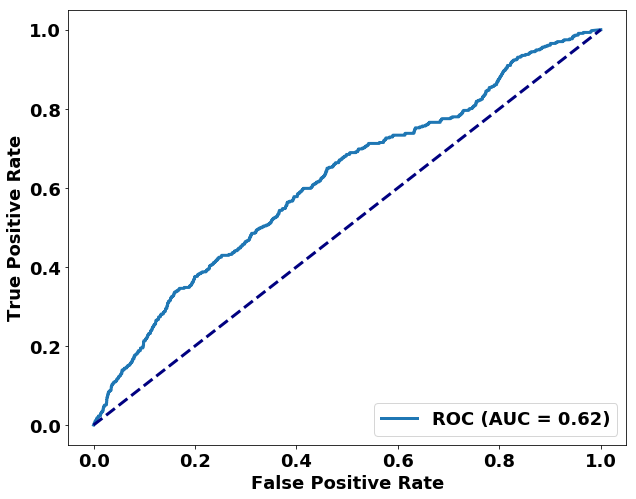
\includegraphics[trim=0in 0.1in 0.1in 0.in,clip,width=1.0\textwidth]{figures/roc_init.png}
\end{minipage}\qquad
\hspace{2ex}
\begin{minipage}[b]{.4\textwidth}
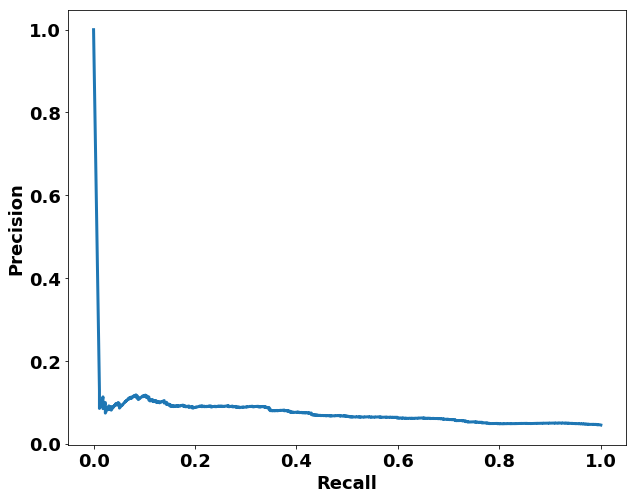
\includegraphics[trim=0in 0.1in 0.1in 0.in,clip,width=1.0\textwidth]{figures/prc_init.png}
\end{minipage}
\caption{ROC (left) and PR (right) curves for KNN model for the initial classifier. 
The PR curve shows that precision is low regardless of recall, 
indicating that we need more data.\label{fig:knn_init}}
\end{figure*}

\begin{figure*}
\centering
\begin{minipage}[b]{.4\textwidth}
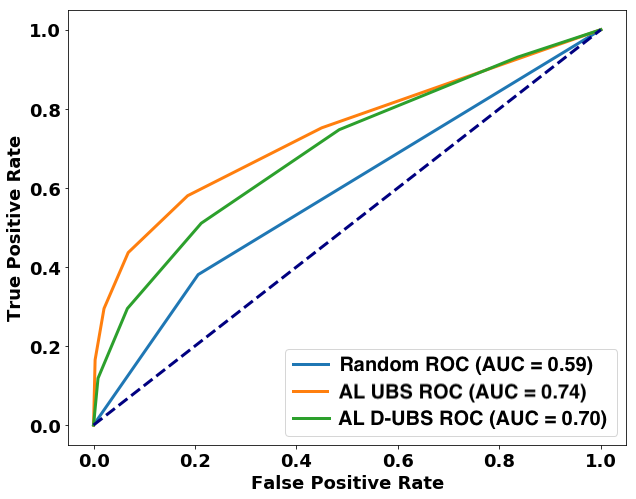
\includegraphics[trim=0in 0.1in 0.1in 0.in,clip,width=1.0\textwidth]{figures/rocs_round5_new.png}
\captionsetup{labelformat=empty}
\label{fig:rocs_round5}
\end{minipage}\qquad
\hspace{2ex}
\begin{minipage}[b]{.4\textwidth}
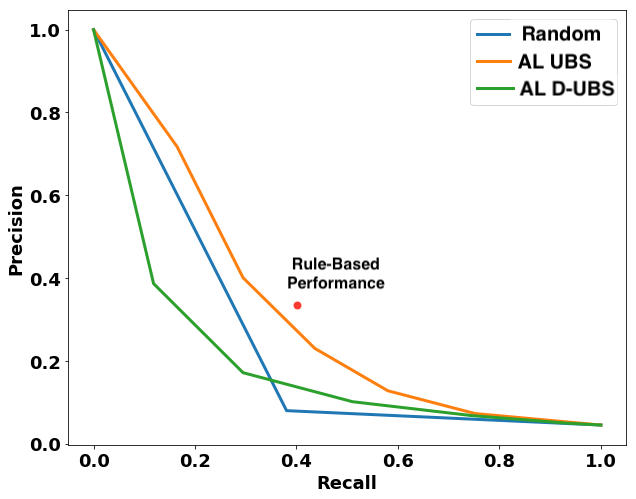
\includegraphics[trim=0in 0.1in 0.1in 0.in,clip,width=1.0\textwidth]{figures/prcs_round5_rule.png}
\captionsetup{labelformat=empty}
\end{minipage}
\caption{ROC (left) and PR (right) curves after four rounds. 
The ROC curves for two active learning strategies, UBS and Distance UBS, show significant improvements,
achieving AUCs of 0.74 and 0.70, respectively: significantly better than the 0.62 achieved by the initial
classifier in Figure~\ref{fig:knn_init}. 
Random, in contrast, performs poorly, with an AUC of just 0.59.
%\ian{I don't understand what you mean here. It is doing better than random. It seems to me that, in general, you are using this graph to make a number of assertions about improvement over initial performance that are not supported by the graph, because you do not show the lines for ``initial performance." All the graph shows is that they all do better than random, with UBS better than Distance UBS, which is in turn better than Random.} 
PR curves also show improvements relative to the initial classifier, with all three strategies
lifting away from the bottom corner, indicating discriminative capacities.
In both types of plots, UBS outperforms Distance UBS. % and approaches rule-based performance.
% AL-1 refers to active learning using NLP-filtered nouns. AL-2 refers to active learning using candidates deemed similar to representative entities.  %\logan{<soapbox>Is it standard practice to use such uninformativ figure captions in CS? I was taught to make the captions almost standalone from the text</soapbox>}
%\ian{I commented out the text that UBS ``approaches rule-based performance'' because the figure does not show that:
%it has no information about rule-based performance.}\roselyne{right! If I add the point, I'll put it back}
}\label{fig:rocs_prcs_round5}\label{fig:prcs_round5}
\end{figure*}

\subsection{Comparing Sampling Strategies}
After the initial round of labeling, we experiment with the three sampling strategies described in Section~\ref{sect:apner_architecture}: Random, UBS, and Distance UBS,
performing four rounds of active learning for each.
Results, in Table~\ref{tab:pr_table}, show
no improvement in the first two rounds for any strategy: % of active learning or the first three rounds of labeling. 
precision remains under 5\% for all.
However, in the third round, we observe increases in precision,
an improvement that  
is sustained in the fourth round for UBS.
Figure~\ref{fig:rocs_prcs_round5} shows ROC and PR curves for the three strategies after four rounds. 
The AUC for UBS is 0.74 and that of Distance UBS is 0.70. 
The PR curves for both are improved (lifting away from the lower left corner of the graph) over the first round, 
with active learning performing better with UBS than with Distance UBS.
%After round 3 and 4, we observe and confirm some, albeit moderate, level context-based predictive ability.
%We also determine that the classifier, which uses UBS is performing better than with the two other strategies.
When tested against our gold standard of 467 one-word polymer names, 
the KNN classifier achieves 18.2\% precision and  45.6\% recall. 

We conclude that while the sampling step
helps insure that the classes are balanced in the initial batch of labels, 
restricting ourselves to just distance candidates, as is done by Distance UBS, does not yield better results than using active learning with all NLP-filtered candidates (UBS).
Intuitively, basic UBS can find \textit{useful} instances (target and non-targets) to be labeled from the entire word embedding space, 
while examples from Distance UBS are clustered around the seed entities that may be collocated in that space.

%\logan{I think the table would be better suited as a plot}\roselyne{I am tempted to remove it, and just indicate that there was not much learning in the first 3 rounds, but Kyle had a comment that people like to see it for themselves and suggested a table. I don't think the plots would look good either has it will bring attention to the problem of using multiple classifiers as previously discussed. I can go back to ommitting this or displaying the last two rounds.}
%\loganfussingaboutrecallandprecision \roselyne{I actually read that this is what people use many times for imbalanced datasets, but I get the point and we have ROCS to got with the last two rounds}

\begin{table}[ht!]
\centering
\caption{Precision and recall relative to the gold standard for
the initial classifier (round 0) and the classifiers trained also with the increased data obtained in each of
four learning rounds, 1--4.\label{tab:pr_table}
}
\vspace{2ex}
%[35.55, 37.69, 46.9, 47.97, 46.47, 48.39, 46.68, 36.4]
\setlength\tabcolsep{6pt}
%\begin{tabular}{*4c}
\begin{tabular}{|c| l | r | r | r |}
\hline
& & \multicolumn{3}{c|}{\textbf{Strategy}} \\
 \textbf{Round} & \textbf{Metric} & \textbf{Random} & \textbf{UBS}  & \textbf{Distance UBS}  \\
%\hline
%Round 0\ \ & \multicolumn{3}{c|}{} \\
\hline
\multirow{2}{*}{0} & Precision &        \multicolumn{3}{c|}{6.53\%} \\
 & Recall\ \ \ \ \ &               \multicolumn{3}{c|}{19.10\%} \\
%\hline
%Round 1\ \  & \multicolumn{3}{c|}{} \\
\hline
\multirow{2}{*}{1}  & Precision     & 3.75\%       &      3.18\%      &  \textbf{5.28\%} \\
 & Recall\ \ \ \ \ & 0.29\%      &   \textbf{93.62\%}     &  56.81\% \\
%\hline
%Round 2\ \  & \multicolumn{3}{c|}{} \\
\hline
\multirow{2}{*}{2} & Precision      & 1.49\%           &      3.79\%      &  \textbf{5.35\%} \\
& Recall\ \ \ \ \ & 1.45\%           &    \textbf{46.38\%}      &  10.14\% \\
%\hline
%Round 3\ \  & \multicolumn{3}{c|}{} \\
\hline
\multirow{2}{*}{3}  & Precision      & 6.02\%              &    \textbf{21.23\%}      &  3.93\% \\
 & Recall\ \ \ \ \ & 44.64\%            &    40.00\%      &  \textbf{84.35\%}  \\
%\hline
%Round 4\ \  & \multicolumn{3}{c|}{} \\
\hline
\multirow{2}{*}{4} & Precision     & 7.06\%          &    \textbf{18.21\%}      &  7.20\% \\
& Recall\ \ \ \ \ & 40.70\%         &     45.64\%     &  \textbf{51.88\%} \\
\hline
\end{tabular}
\end{table}

We selected seed entities based on their frequency in our corpus. %and the yield of target entities during sampling.%\ian{I thought that you said above that you picked the most frequent words?}\roselyne{Yes, but we also experimented with them, top, vs, top3, vs top10, but it is not necessary.}
This observation suggests that we could also study how the choice of seed entities impact of the performance of the classifier during the active learning process. 
We revisit this concept of \textit{diversity} of labels in the Section~\ref{sec:discussion}. 
Note that with limited training data and based solely on context, the classifier retrieves 45.6\% (more than one third) of the gold standard polymers with a precision of 18.2\%, after five hours of expert labeling. 
For comparison, an attempt to extract polymer names using the rule: 
\textit{if the name contains ``poly'' extract it as a polymer}, gets recall of 41\% and precision of 34\% on the same dataset.
We conclude that with our relatively small dataset, we are able to achieve close to rule-based performance, 
using active learning and little labeling.
%\logan{I think we should show this point on the plot for context. Also, state what you conclude from the comparison. Don't leave it up to the reader to state the conclusion.}

%\subsection{Using Active Learning Labels with Character-Level Enhanced Embeddings}
\subsection{Active Learning Labels + Character-Level Embeddings}
\label{sec:results}
After just 1000 labels, the context-based classifier using active learning applied to NLP-filtered candidates achieved performance comparable to rule-based performance, 
but not quite to the polymer-enhanced CDE+.
With the goal of further improving polyNER performance,
we experiment with the use of an alternative word embedding model, FastText, which 
%Next, we train a word embedding model enhanced with sub-word information using polyNER labels. 
%\logan{Why are you doing this? You need some motivation for this section, otherwise it kinds of jumps out of nowhere and begs the question: Why did you not use this through the entire study? Maybe you can say this section is devoted to "further tuning the model now that you have a large-enough pool of data to make selections statistically-reasonable"?}
%We compare the performance to a state-of-the-art chemistry-aware NLP toolkit. 
%and we end with a discussion of the results.
uses word representations enriched with sub-word (character-level) information.
Because FastText considers sub-word information as well as
context, it can consider word morphology differences, such as prefixes
and suffixes. Sub-word information is especially useful for words for which
context information is lacking, as words can still be compared to morphologically similar
existing words. We set the length of the sub-word used for comparison\textemdash
FastText's \texttt{n_gram} parameter\textemdash to five characters, based on our intuition that
many polymers begin with the prefixes ``poly'' or ``poly(.'' 
Therefore, we generate a FastText word embedding model, 
and generate character-enhanced vectors for our UBS-labeled candidates.

%\ian{Next is confusing to me as (it seems to me) you refer to things in roundabout ways:
%e.g., I am not clear what are ``these candidates'' or what it is that is ``identified as best-performing in previous experiments''.}
Next, we train a KNN classifier using vectors for the candidates labeled through active learning from the NLP-filtered candidates (the active learning strategy identified as best-performing in Figure~\ref{fig:prcs_round5}).
%\logan{Confusing. Is UBS not active learning?}\roselyne{it's the sampling method}
We test the classifier against NLP-filtered nouns from our 100-document test set.
KNN classifier performance improves when using these word vectors, 
achieving 29.7\% precision and 81.9\% recall,
%\logan{Why sow both figures if you say PRC is better.}\roselyne{I will end up taking them off, as I'm now at 12 pages}
%In this case, the classifier achieves 29.7\% precision and 81.9\% recall. 
comparable to those achieved by CDE (see Section~\ref{sec:cde}).
% although as CDE aims to extract all
%chemical compounds, not just polymers, it serves only as a demonstration of an
%alternative approach in the absence of a polymer NER system. % (Note that CDE also extracts properties). 
CDE's recall is high
at 74.5\%, but its precision for polymers is, as expected, low at 8.7\%, as it does not incorporate polymer knowledge. 
%\loganfussingaboutrecallandprecision \roselyne{comes with PRC so should be good here}
In Figure~\ref{fig:UBS_prcs_fasttext}, we show the PR curve for the FastText vector classifier
and also results for the polymer-enhanced CDE+
which achieve 42.2\% precision and 68.3\% recall on the same test set.
%\ian{rewording ok here?}\roselyne{yes}
%We show the PR curve for the FastText vector classifier and the CDE+ performance in Figure
%as shown in Figure~\ref{fig:UBS_prcs_fasttext}.\ian{Is this a good place for figure reference?}
We achieve higher recall than CDE and CDE+ using labels from UBS and FastText vectors 
and in-between (higher than CDE and lower than CDE+)
%\ian{I don't know how to interpret this word.}\roselyne{I thought that would be better "than in-between" precision}
precision.%, with only about five hours of expert labeling.

\subsection{Discussion and Future Work}
\label{sec:discussion}
We have previously used seed entities to bootstrap classifiers of context-based word vectors. 
Using an ensemble of classifiers, polyNER allowed users to tradeoff precision and recall.
In this attempt to improve performance, while efficiently using experts' time, we used active learning to obtain more labels. %\roselyne{Repeating again, may need to remove.}
However, we do not observe an increase of precision over the 5\% fraction of polymers until the third round of active learning with NLP-filtered words (800 labels). 
This suggests that our label batch size is lower than the minimum number of labels necessary to start the learning process.
More detailed study of performance vs. label batch size will help pinpoint the appropriate number of labels and level of bootstrapping required for learning.
We can also ask the following questions: Could we achieve CDE performance classifying only context-based (not character enhanced) representation? If so, how many more iterations would it take? If not, how much do we need to increase the size and/or improve our current corpus of \num{1690} documents?
Corpora for NER tasks are curated and typically include sentences with one or more entities.
We could investigate other semi-supervised method to eliminate negative sentences from our corpus (e.g. labeling sentences and classification of sentence vectors for example).

PolyNER achieves CDE performance using labels obtained via active learning (UBS sampling strategy) and FastText vectors.
We attribute the increased performance to the character embedding enhancement, which not only recognizes ``poly'' (and yields more names based on this n-gram comparison), 
but also filters out more anomalous candidates (preceding or following polymer names) generated during tokenization and missed by the filtering steps, 
such as ``\textit{$A_mB_n$}'' and ``\textit{Mw/Mn=1.36}.'' 
In other words, the classifiers of character and (context-based) word embedding vectors perform better than classifiers of only context-based word embedding.
Given this result, one may wonder whether the active learning process itself could benefit from using this enhanced vector embedding. 
To determine whether this is the case,
we repeated the active learning experiment using the entire corpus of NLP-filtered candidates and classifying FastText (enhanced) vectors instead of Gensim vectors at each round. 
However, performance was worse than random.
%the classifier's ROC curve did not achieve CDE performance after five rounds and was below random performance.%\logan{Wasn't it also worse than the randomly-selected words?}\roselyne{yes, but doesn't it make you want to see another figure more}

These results suggest that character-level information enhances classifier performance only once a certain threshold of context information has been captured by the embedding.
We explain this observation as follows. 
In FastText, the portion of the word embedding vector generated by using context varies depending on how much context is available in the entire corpus. 
For words deemed to have enough context, vectors do not include any character-level information. 
At the other extreme, for previously unseen words, the embedding is generated based solely on character n-gram information and comparison to other words in the corpus.
During the active learning process, candidates to be labeled by experts are selected by using maximum-entropy-based uncertainty sampling: that is, words for which prediction probability is similar for target and non-target.
Such candidates are more likely to lack context
and thus have vectors that use mostly character-level information.
%When all or most of the word embedding vector 
As a result, the expert is often presented with nearly identical candidates (e.g., PS13k/PMMA12k, PS214k/PMMA12k, PS31.6k/PMMA12k), which hinders the learning process as these candidates are located in close vicinity in terms of the full (character and context) word embedding space.
In other words, in this full space, while their uncertainty measure is comparable, these examples are not \textit{diverse}, where diversity is a measure of the distance of the examples to each other or previously labeled instances~\cite{brinker2003incorporating}.
One solution to explore in future work would be to impose a diversity constraint on the candidates,
for example by using batch active learning~\cite{settles2009active}.
%\logan{There are batch active learning papers, and surely a review. Cite one so that people do not think you're planning to reinvent such methods.}\roselyne{Definitely planned on adding citation but hadn't reread that part, thanks}
%\logan{This seem more like a "Future Work/Can we do even better!?" section than an actual discussion. Should we rename the section accordingly}


%\begin{figure}[H]
\begin{figure}
\centering
%\begin{minipage}[b]{.4\textwidth}
%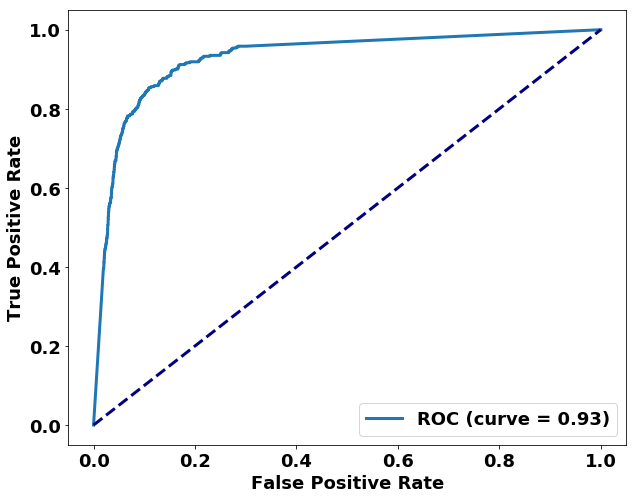
\includegraphics[trim=0in 0.1in 0.1in 0.in,clip,width=3.5in]{figures/fasttext_roc_al_corpus_round5_100}
%\caption{ROC curve for KNN model trained using active learning labels and word representations enriched with character-level information.}\label{fig:UBS_rocs_fasttext}
%\end{minipage}\qquad
%\begin{minipage}[b]{.4\textwidth}
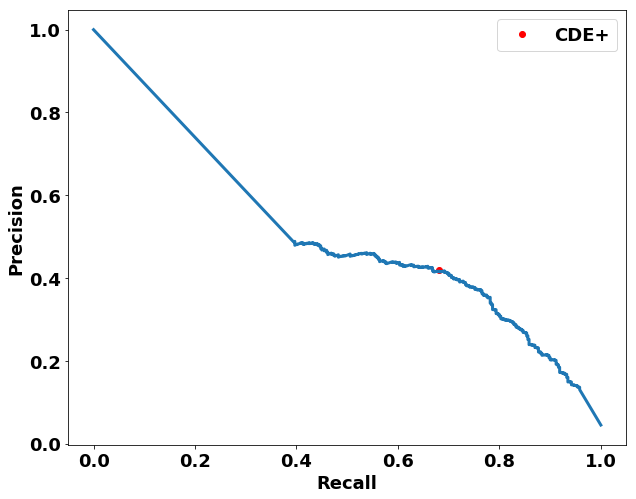
\includegraphics[trim=0in 0.1in 0.1in 0.in,clip,width=3.5in]{figures/fasttext_prc_al_corpus_round5_100}
\caption{PR curve for KNN model trained with active learning labels and word representations enriched with character-level information. Results for CDE+ are also shown. 
\ian{I'd be interested in Kyle's views, but I feel that we need some explanation of why the line is straight for recall from 0 to 0.4.}
\roselyne{(PR curves, like ROC curves are generated by varying the threshold of probability that separates classes, straight lines indicate that many points have the same probability values, and varying the threshold yield identical precision to recall ratio.) Not sure if this is clear enough.}
}
\label{fig:UBS_prcs_fasttext}
%\end{minipage}
\end{figure}

%\subsection{Labeling}\label{sec:labeling}
%We conduct some experiments to estimate labeling time. 
%We ask two polymer scientists to label 200 candidates from a subset of our corpus.
%One expert reports 30 minutes, the other 45 minutes. We overestimate the time to label 200 candidates at one hour of expert time.
%Based on user feedback, we also improve the labeling Web interface after the above-mentioned test rounds to further facilitate and speed up labeling.
%For example, we increase the number of example sentences available to provide context, to decrease the number of occurrences in which experts have to look up original publications for candidates.
%We also increase the size of checkmarks to make it easier to reject erroneous candidates.
%%Having performed these initial tests, and considering that expert time is expensive, we allow annotators to save their progress and come back to labeling anytime within a week's time. \roselyne{Is this only going to add confusion?}
%In the initial labeling round, we
%we perform crosschecking for 10\% of the batch of labels. 
%We confirm agreement between labels for all but one of 20: an agreement rate of 95\%.









